\chapter{Appendix A}
\renewcommand{\thefigure}{A.\arabic{figure}}
\begin{figure}
    \centering
    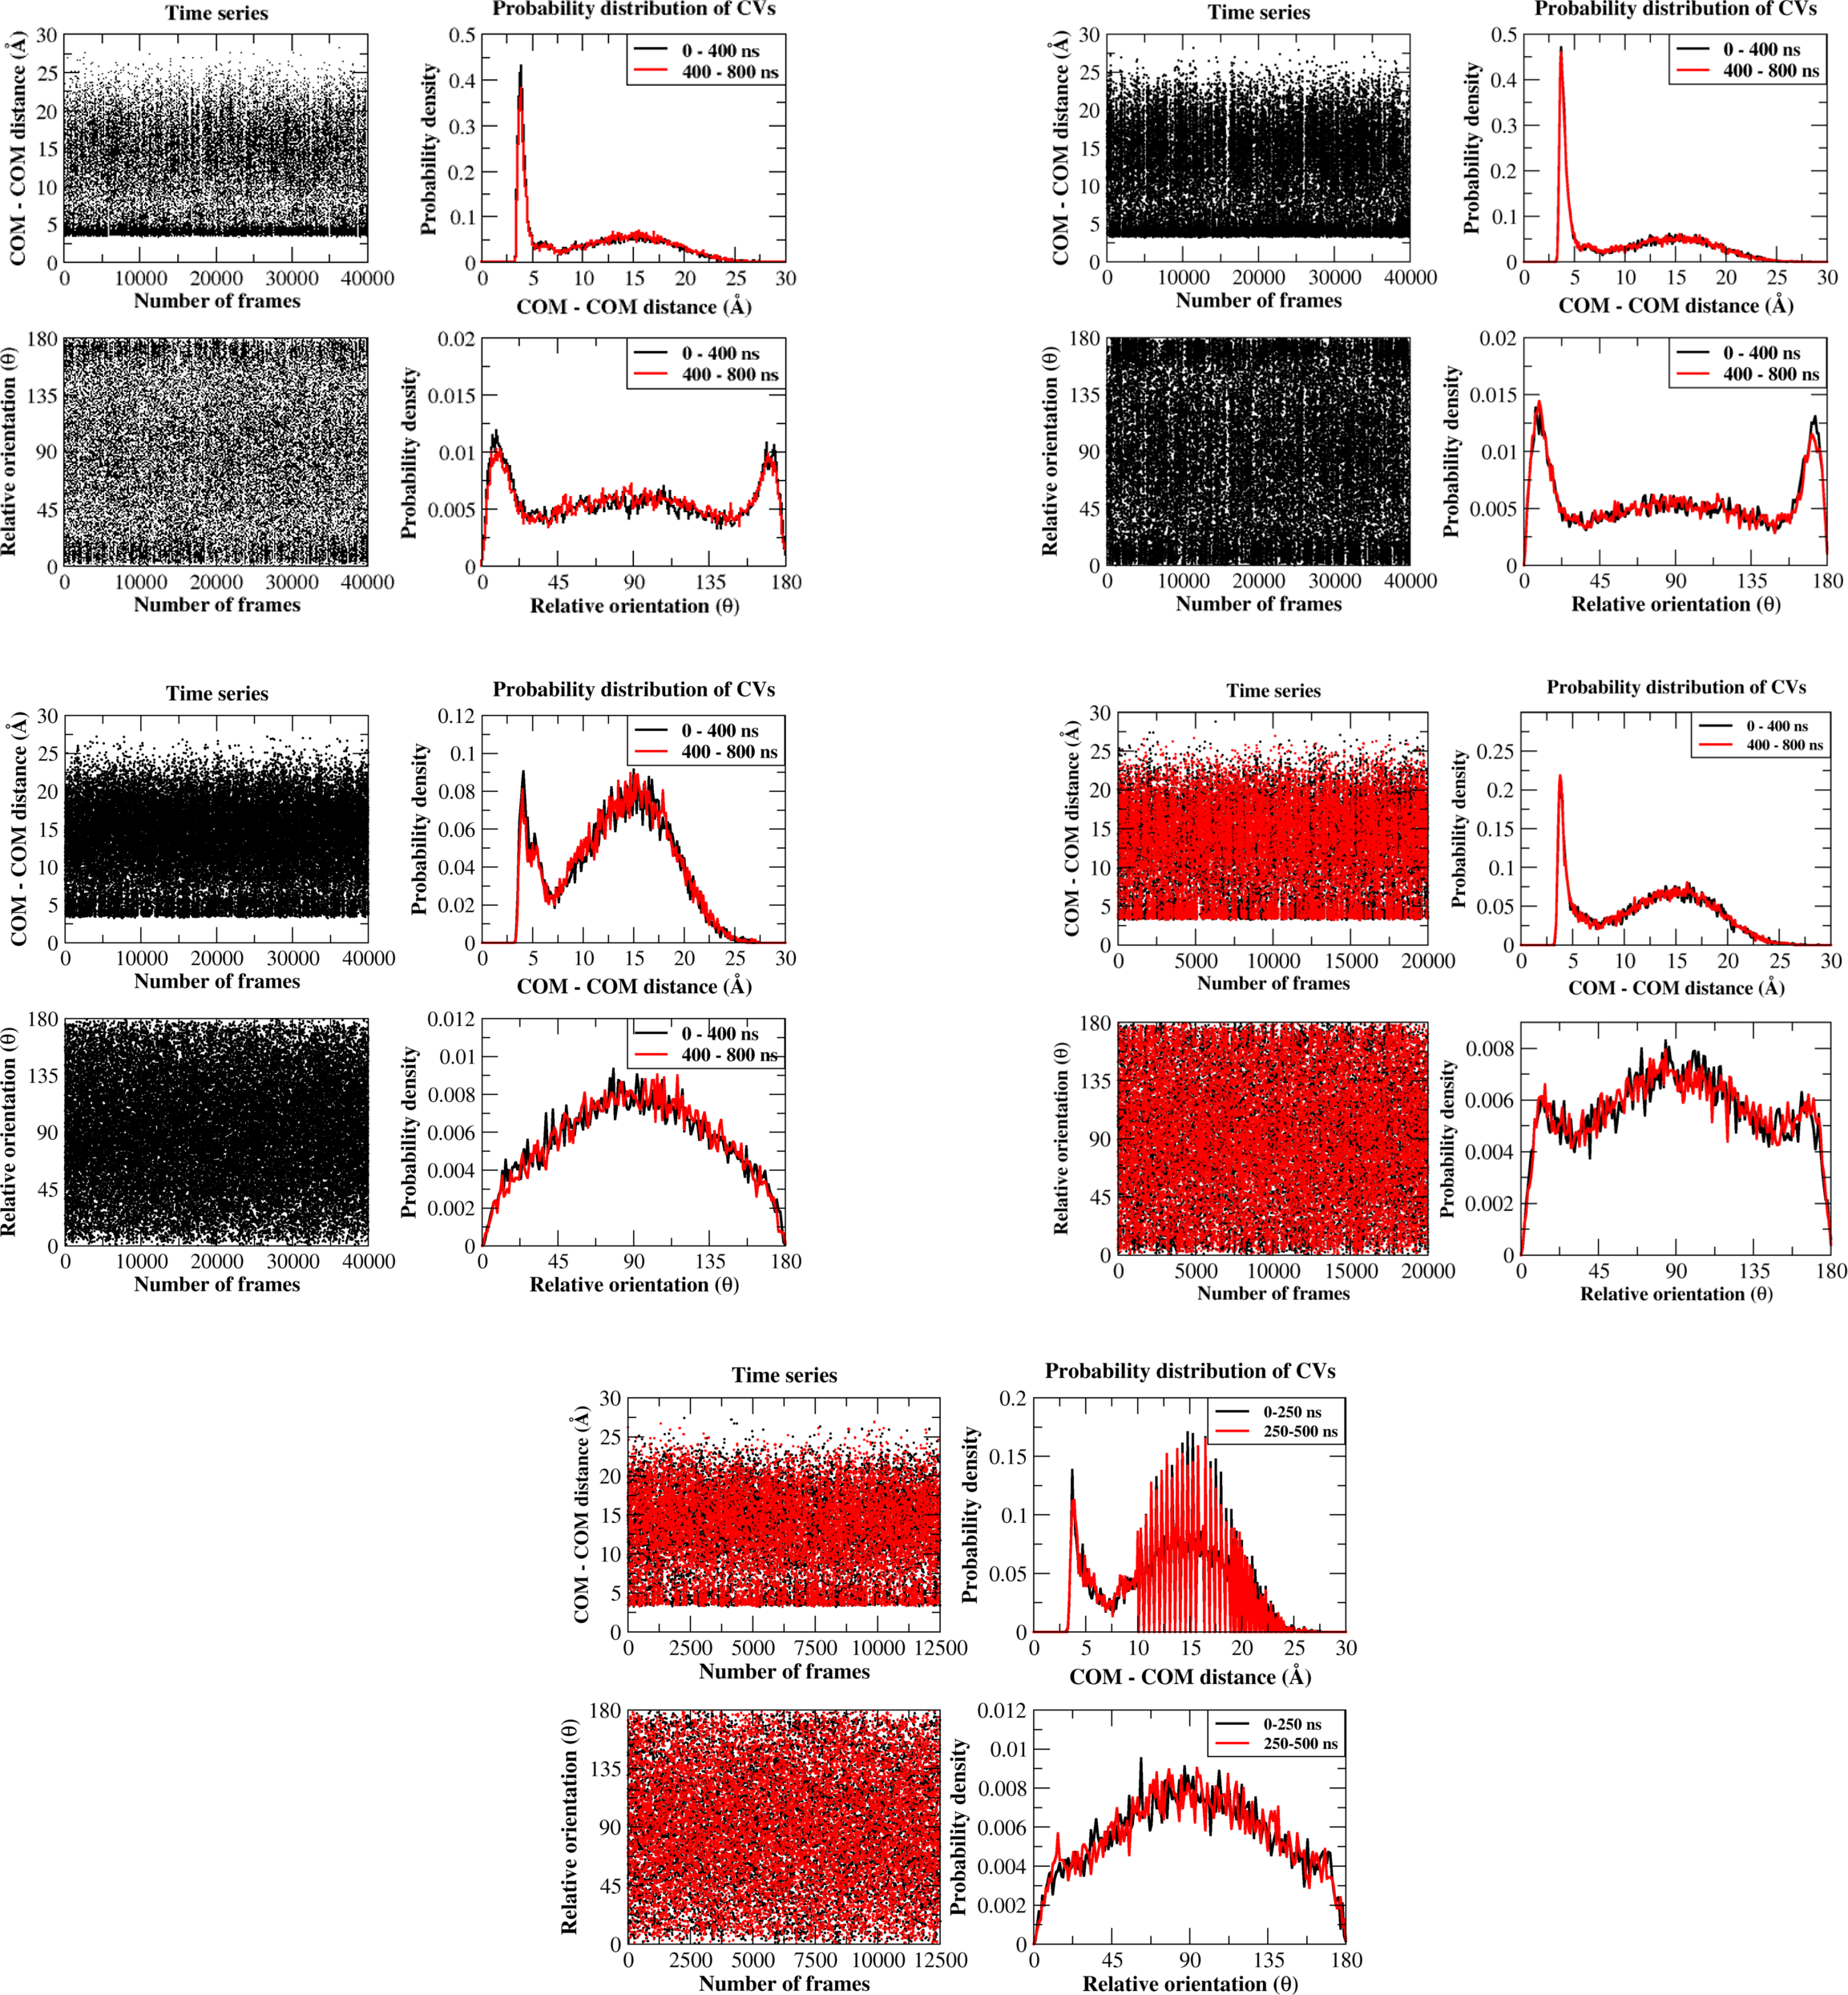
\includegraphics[width=\textwidth]{Appendix/Figures/A1_port.png}
    \caption[Time series plots for the d\textsubscript{Nuc-Nuc} and relative orientations of the nucleobases obtained from additive FF simulations]{Time series plots for the d\textsubscript{Nuc-Nuc} and relative orientations of the nucleobases obtained from additive FF simulations. Distances are presented in units of $\angstrom$ and orientations in ($\degree$)}
\end{figure}

\begin{figure}
    \centering
    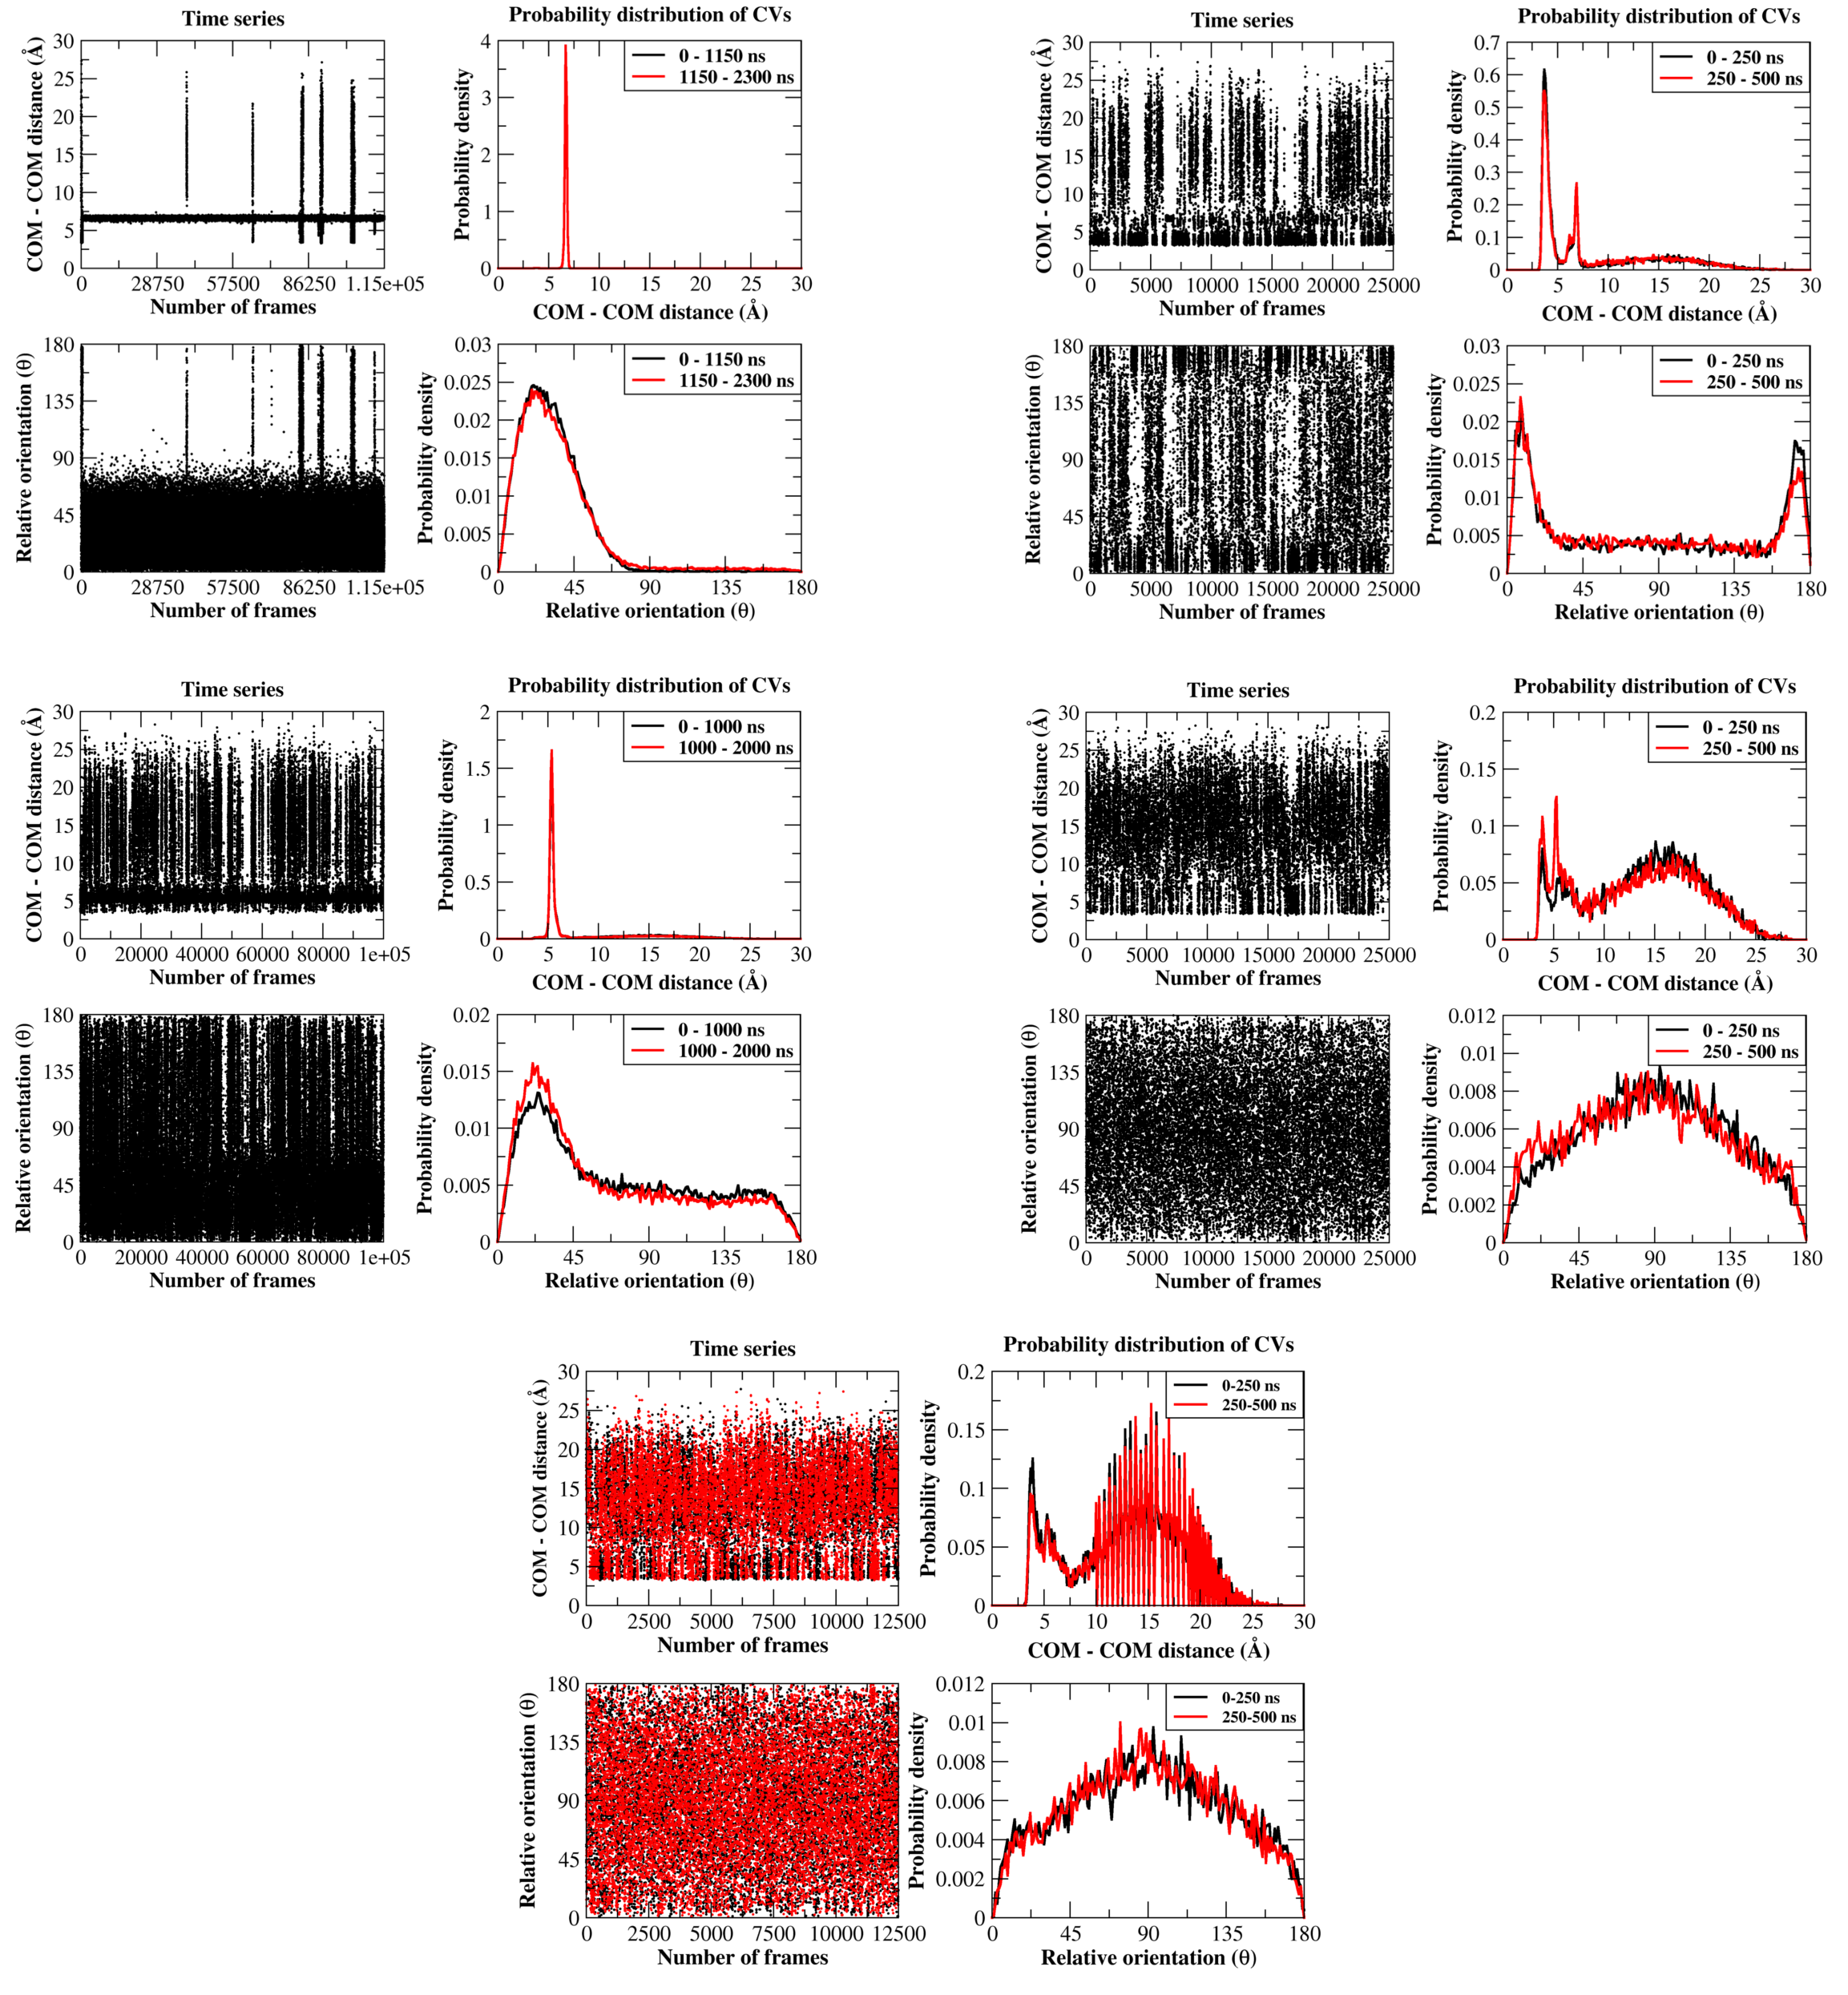
\includegraphics[width=\textwidth]{Appendix/Figures/A2_port.png}
    \caption[Time series plots for the d\textsubscript{Nuc-Nuc} and relative orientations of the nucleobases obtained from Drude polarizable FF simulations]{Time series plots for the d\textsubscript{Nuc-Nuc} and relative orientations of the nucleobases obtained from Drude polarizable FF simulations. Distances are presented in units of $\angstrom$ and orientations in ($\degree$)}
\end{figure}

\begin{figure}
    \centering
    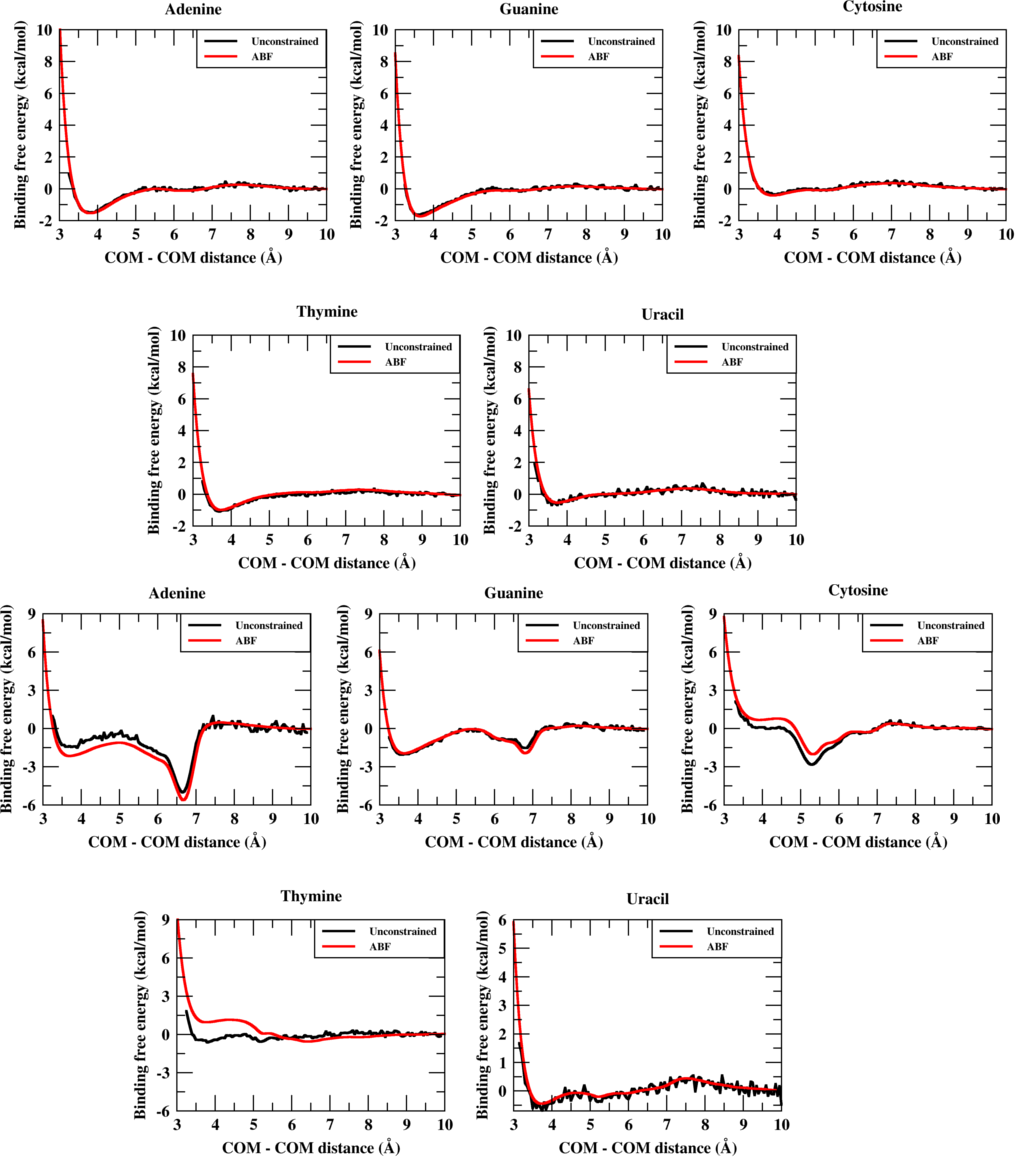
\includegraphics[width=\textwidth]{Appendix/Figures/A3_port.png}
    \caption[Potential of Mean Force (PMF) plots for nucleobase - nucleobase interactions obtained from additive and Drude polarizable FF simulations]{Potential of Mean Force (PMF) plots for nucleobase - nucleobase interactions obtained from additive and Drude polarizable FF simulations. Distances are presented in units of $\angstrom$ and energies are presented in units of kcal/mol.}
\end{figure}

\begin{figure}
    \centering
    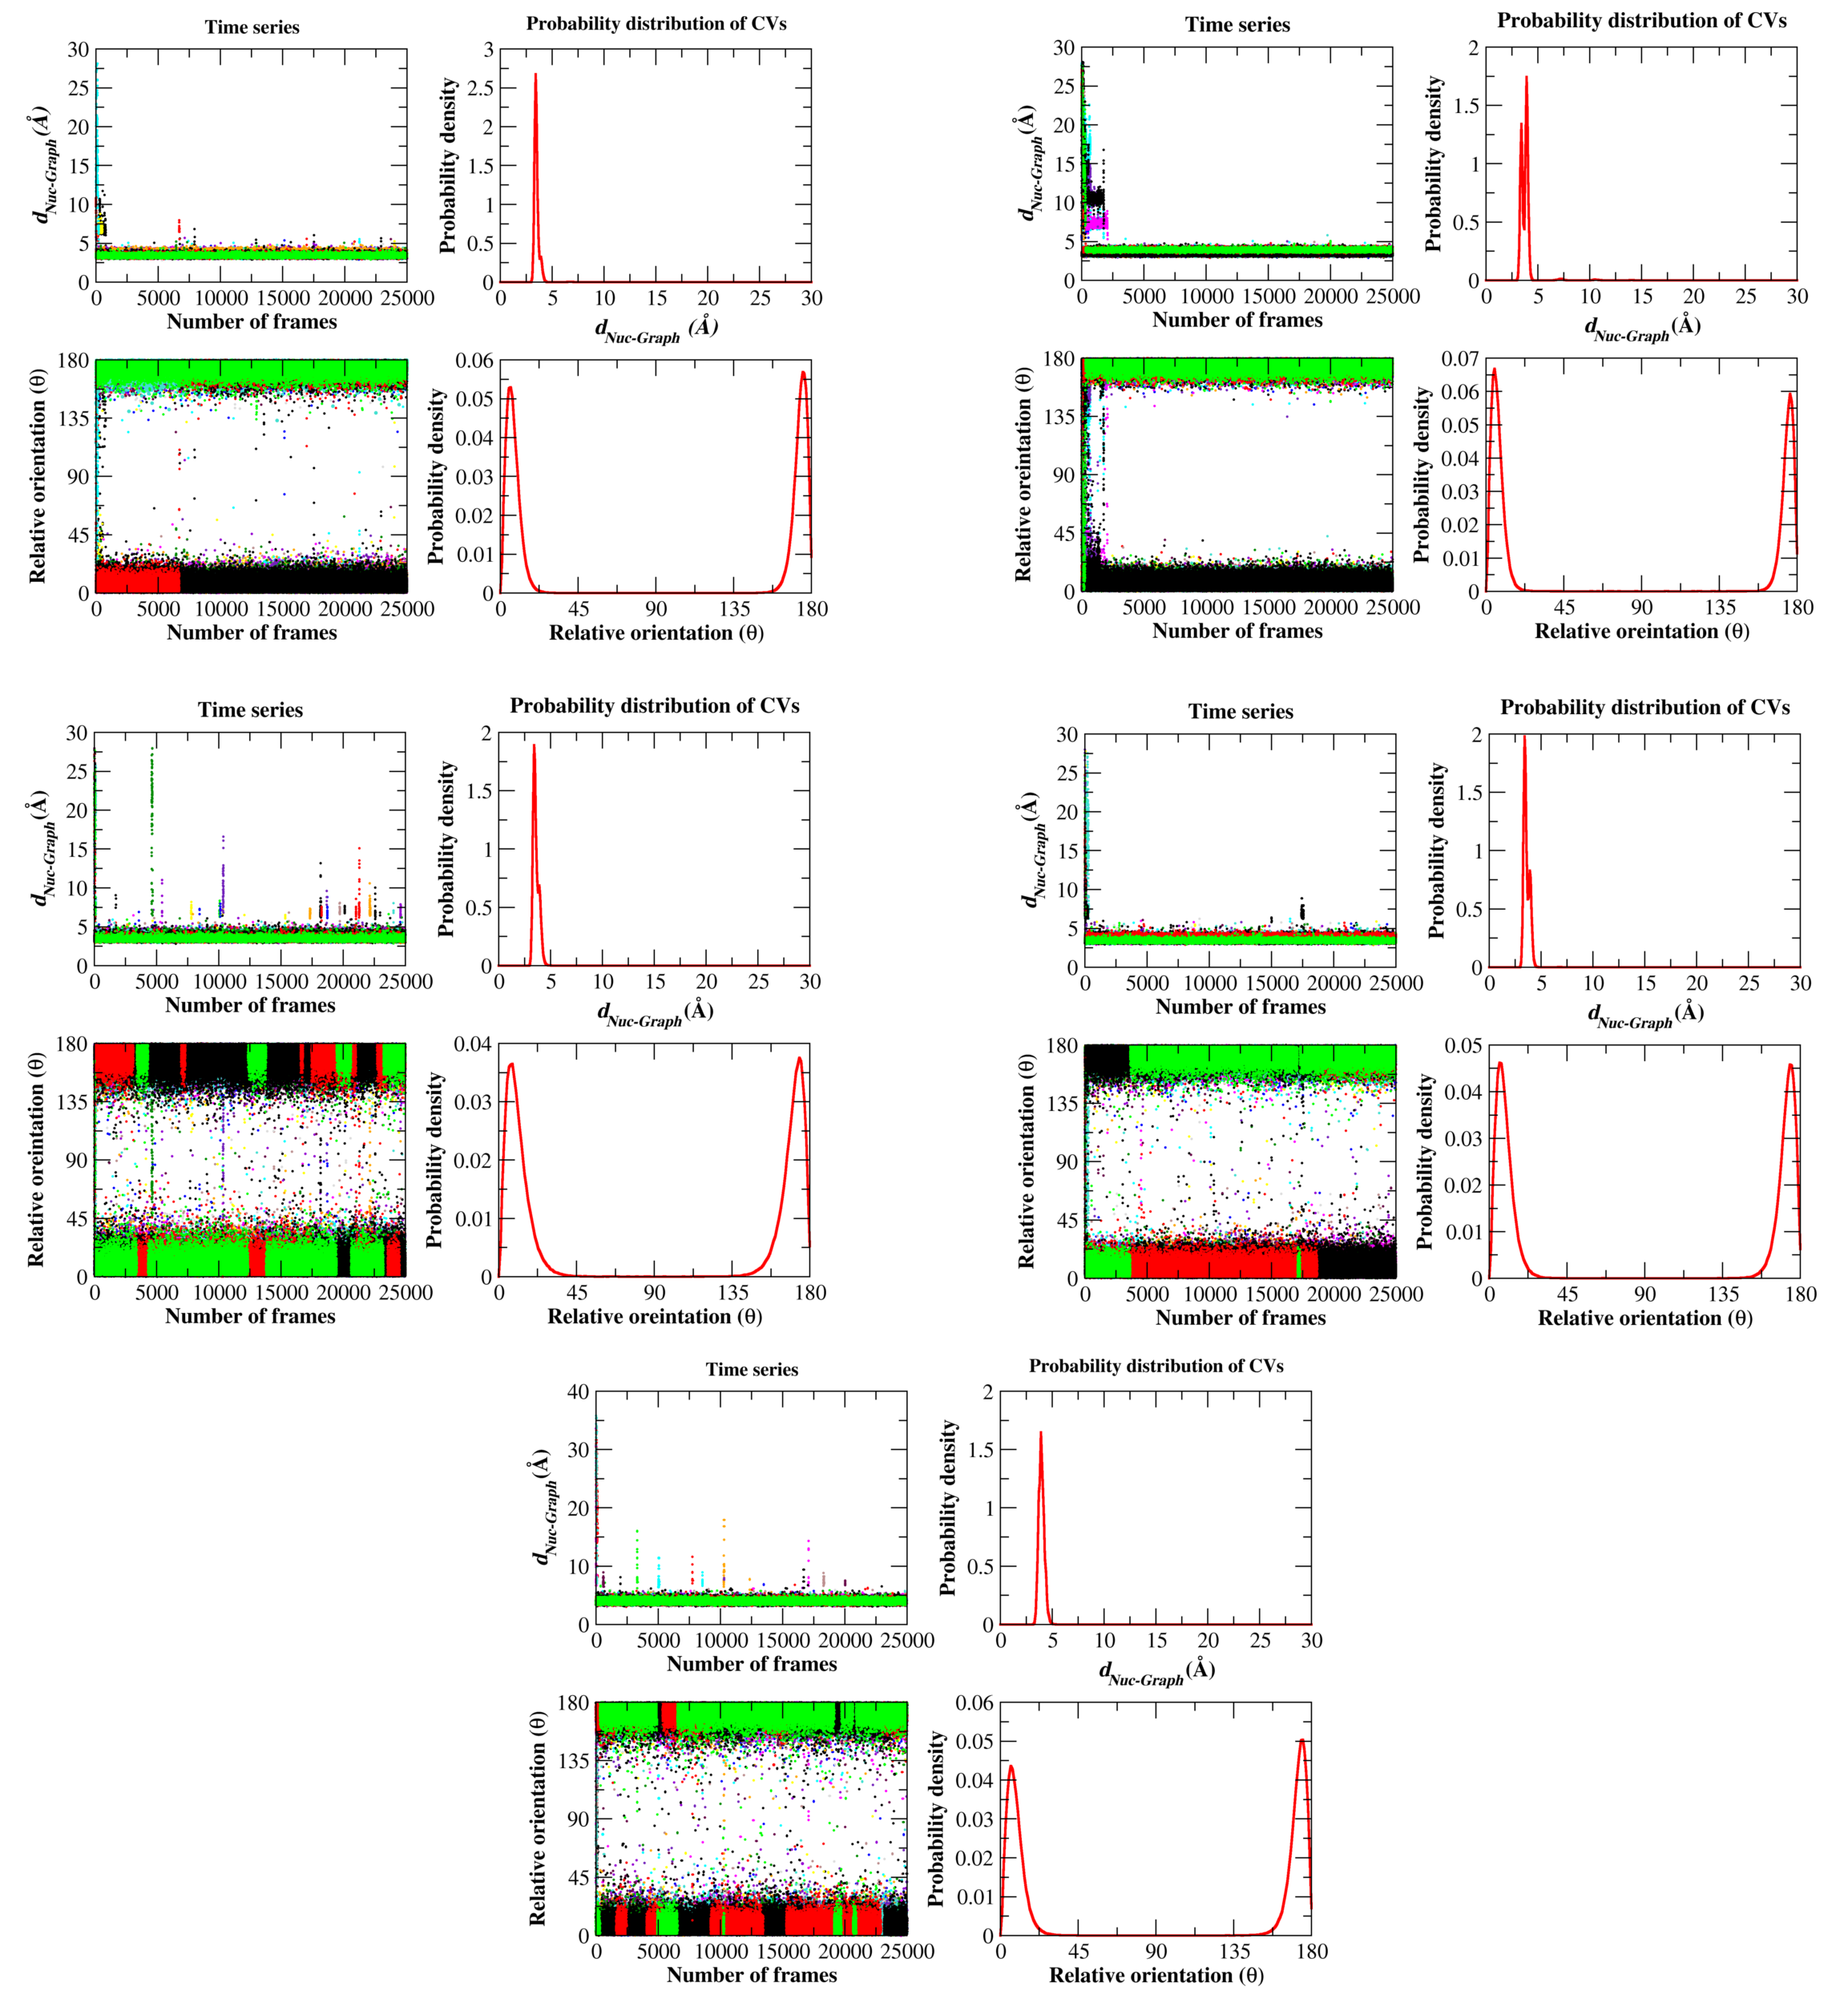
\includegraphics[width=\textwidth]{Appendix/Figures/A4_port.png}
    \caption[Time series plots for the d\textsubscript{Nuc-Graph} and relative orientations of the nucleobases obtained from nucleobase - graphene additive FF simulations]{Time series plots for the d\textsubscript{Nuc-Nuc} and relative orientations of the nucleobases obtained from nucleobase - graphene additive FF simulations. Distances are presented in units of $\angstrom$ and orientations in ($\degree$)}
\end{figure}

\begin{figure}
    \centering
    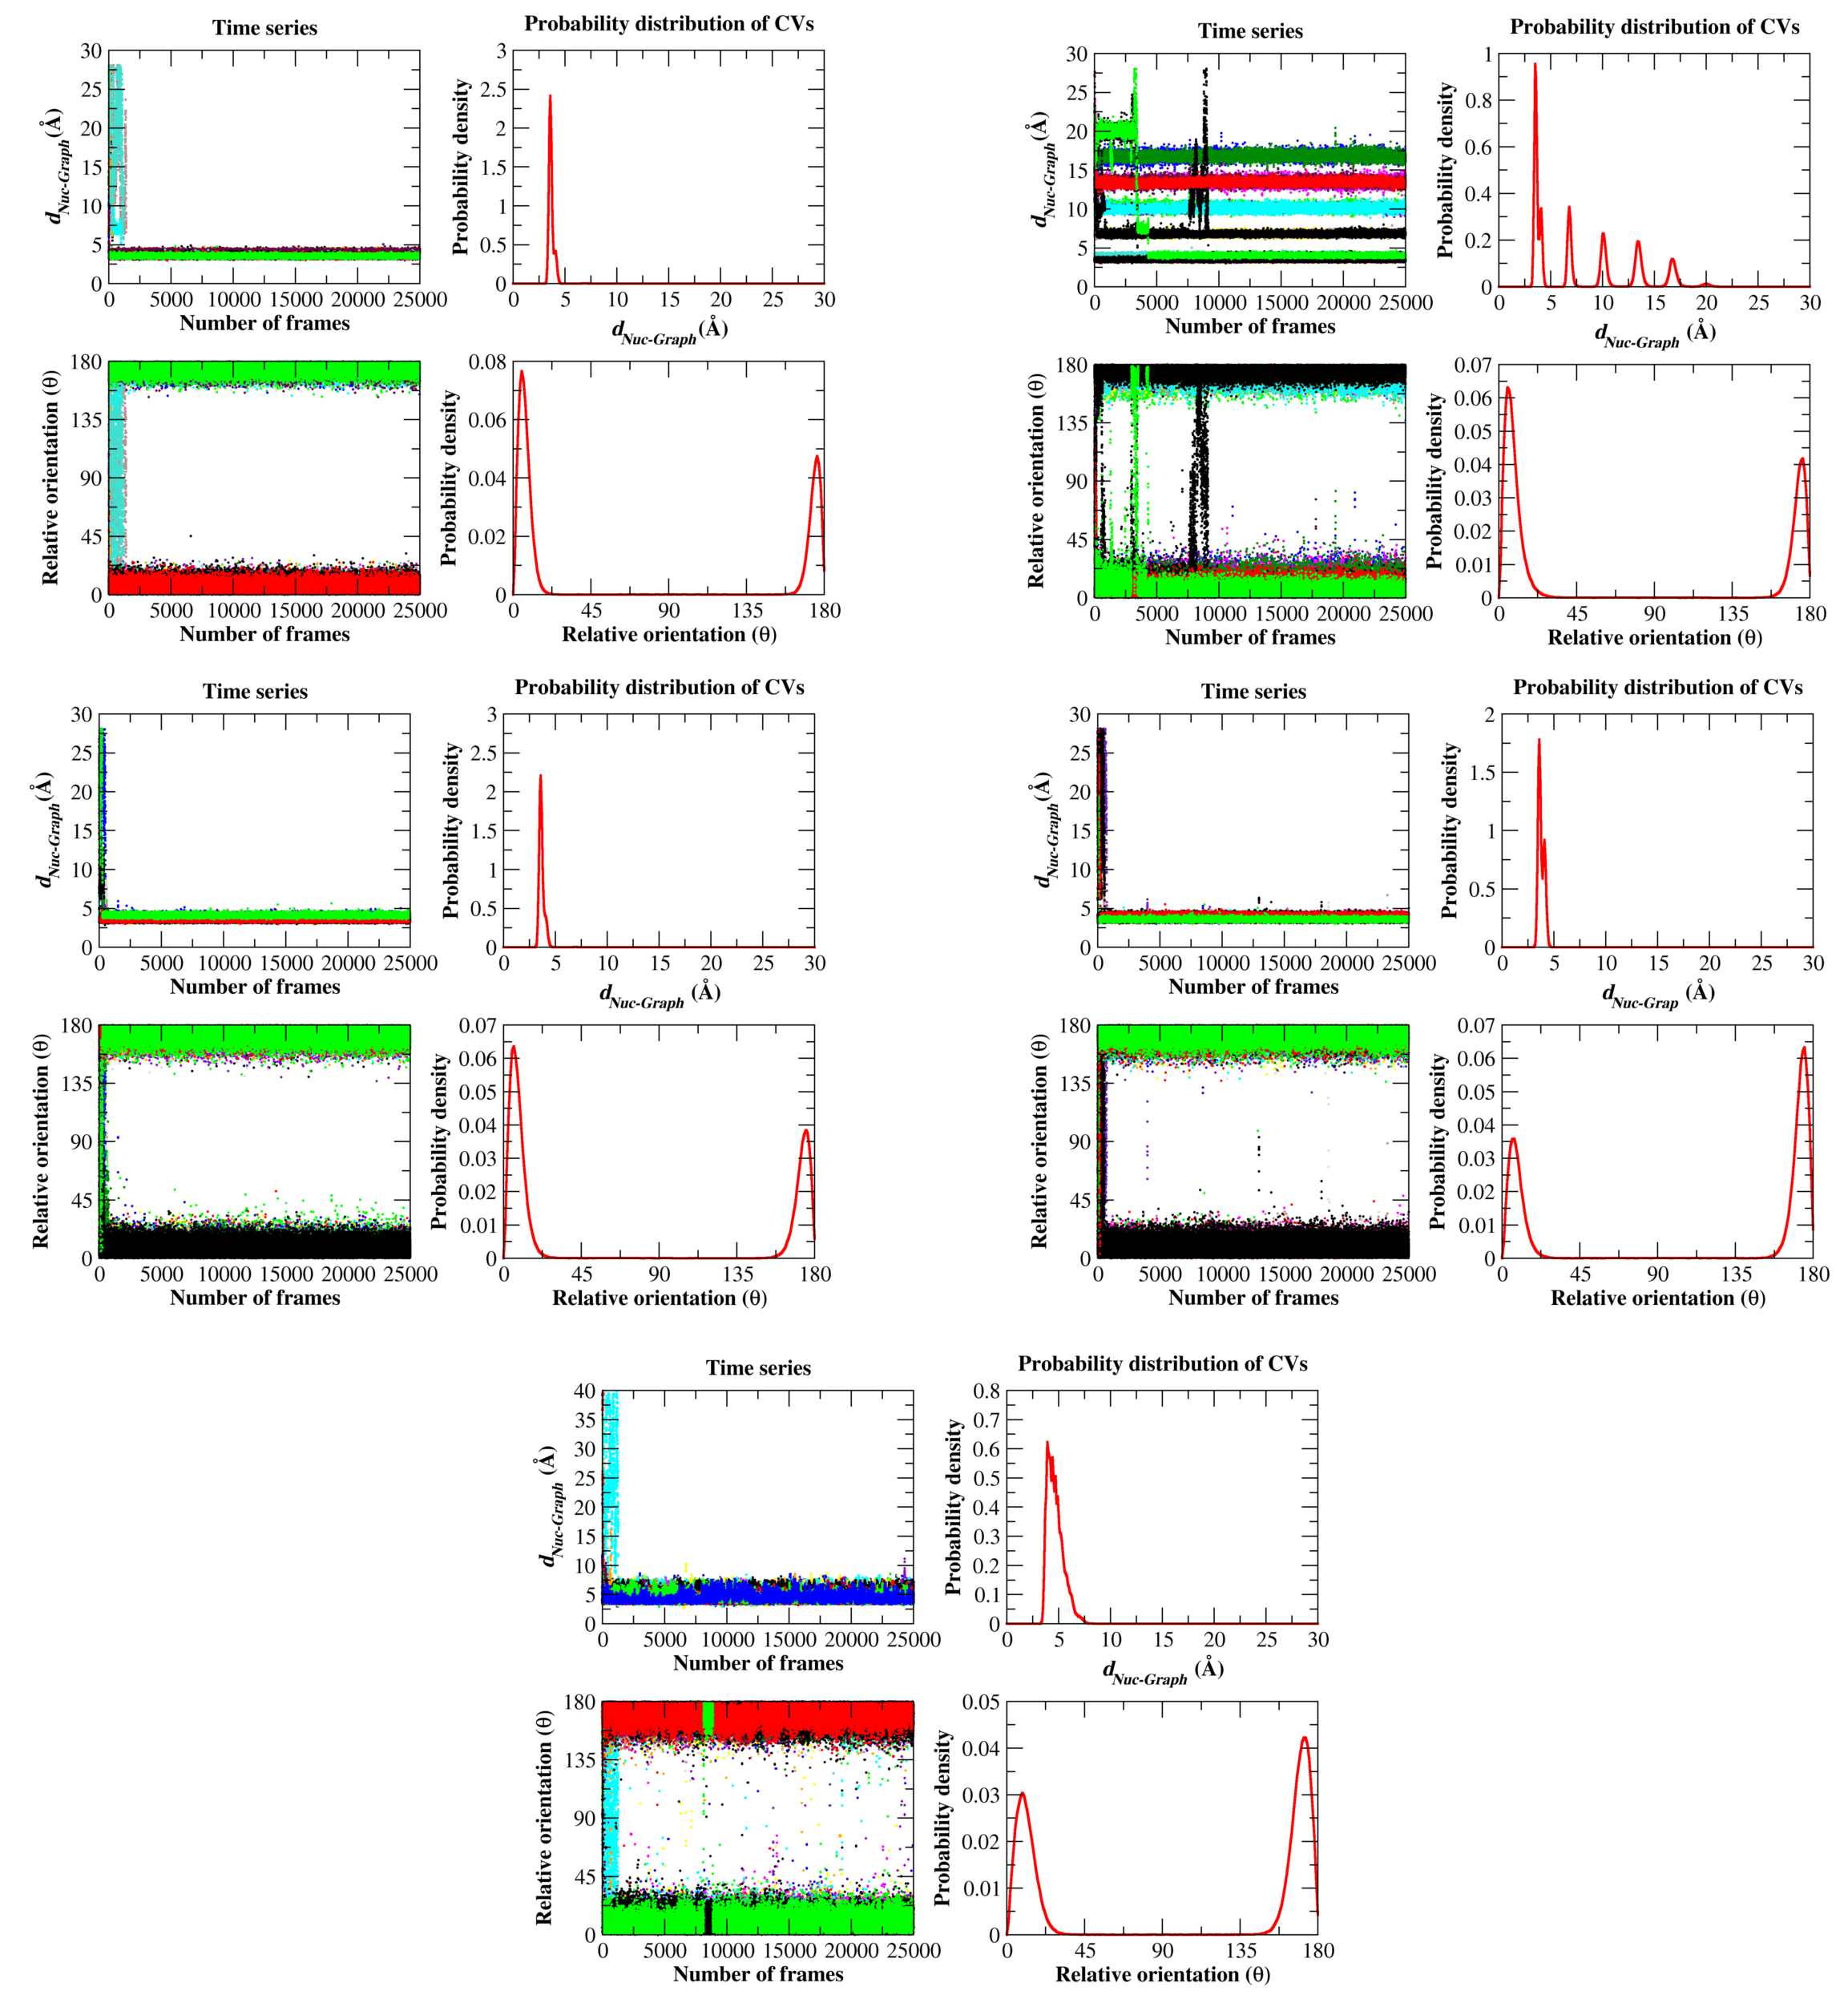
\includegraphics[width=\textwidth]{Appendix/Figures/A5_port.png}
    \caption[Time series plots for the d\textsubscript{Nuc-Graph} and relative orientations of the nucleobases obtained from nucleobase - graphene Drude polarizable FF simulations]{Time series plots for the d\textsubscript{Nuc-Nuc} and relative orientations of the nucleobases obtained from nucleobase - graphene Drude polarizable FF simulations. Distances are presented in units of $\angstrom$ and orientations in ($\degree$)}
\end{figure}

\begin{figure}
    \centering
    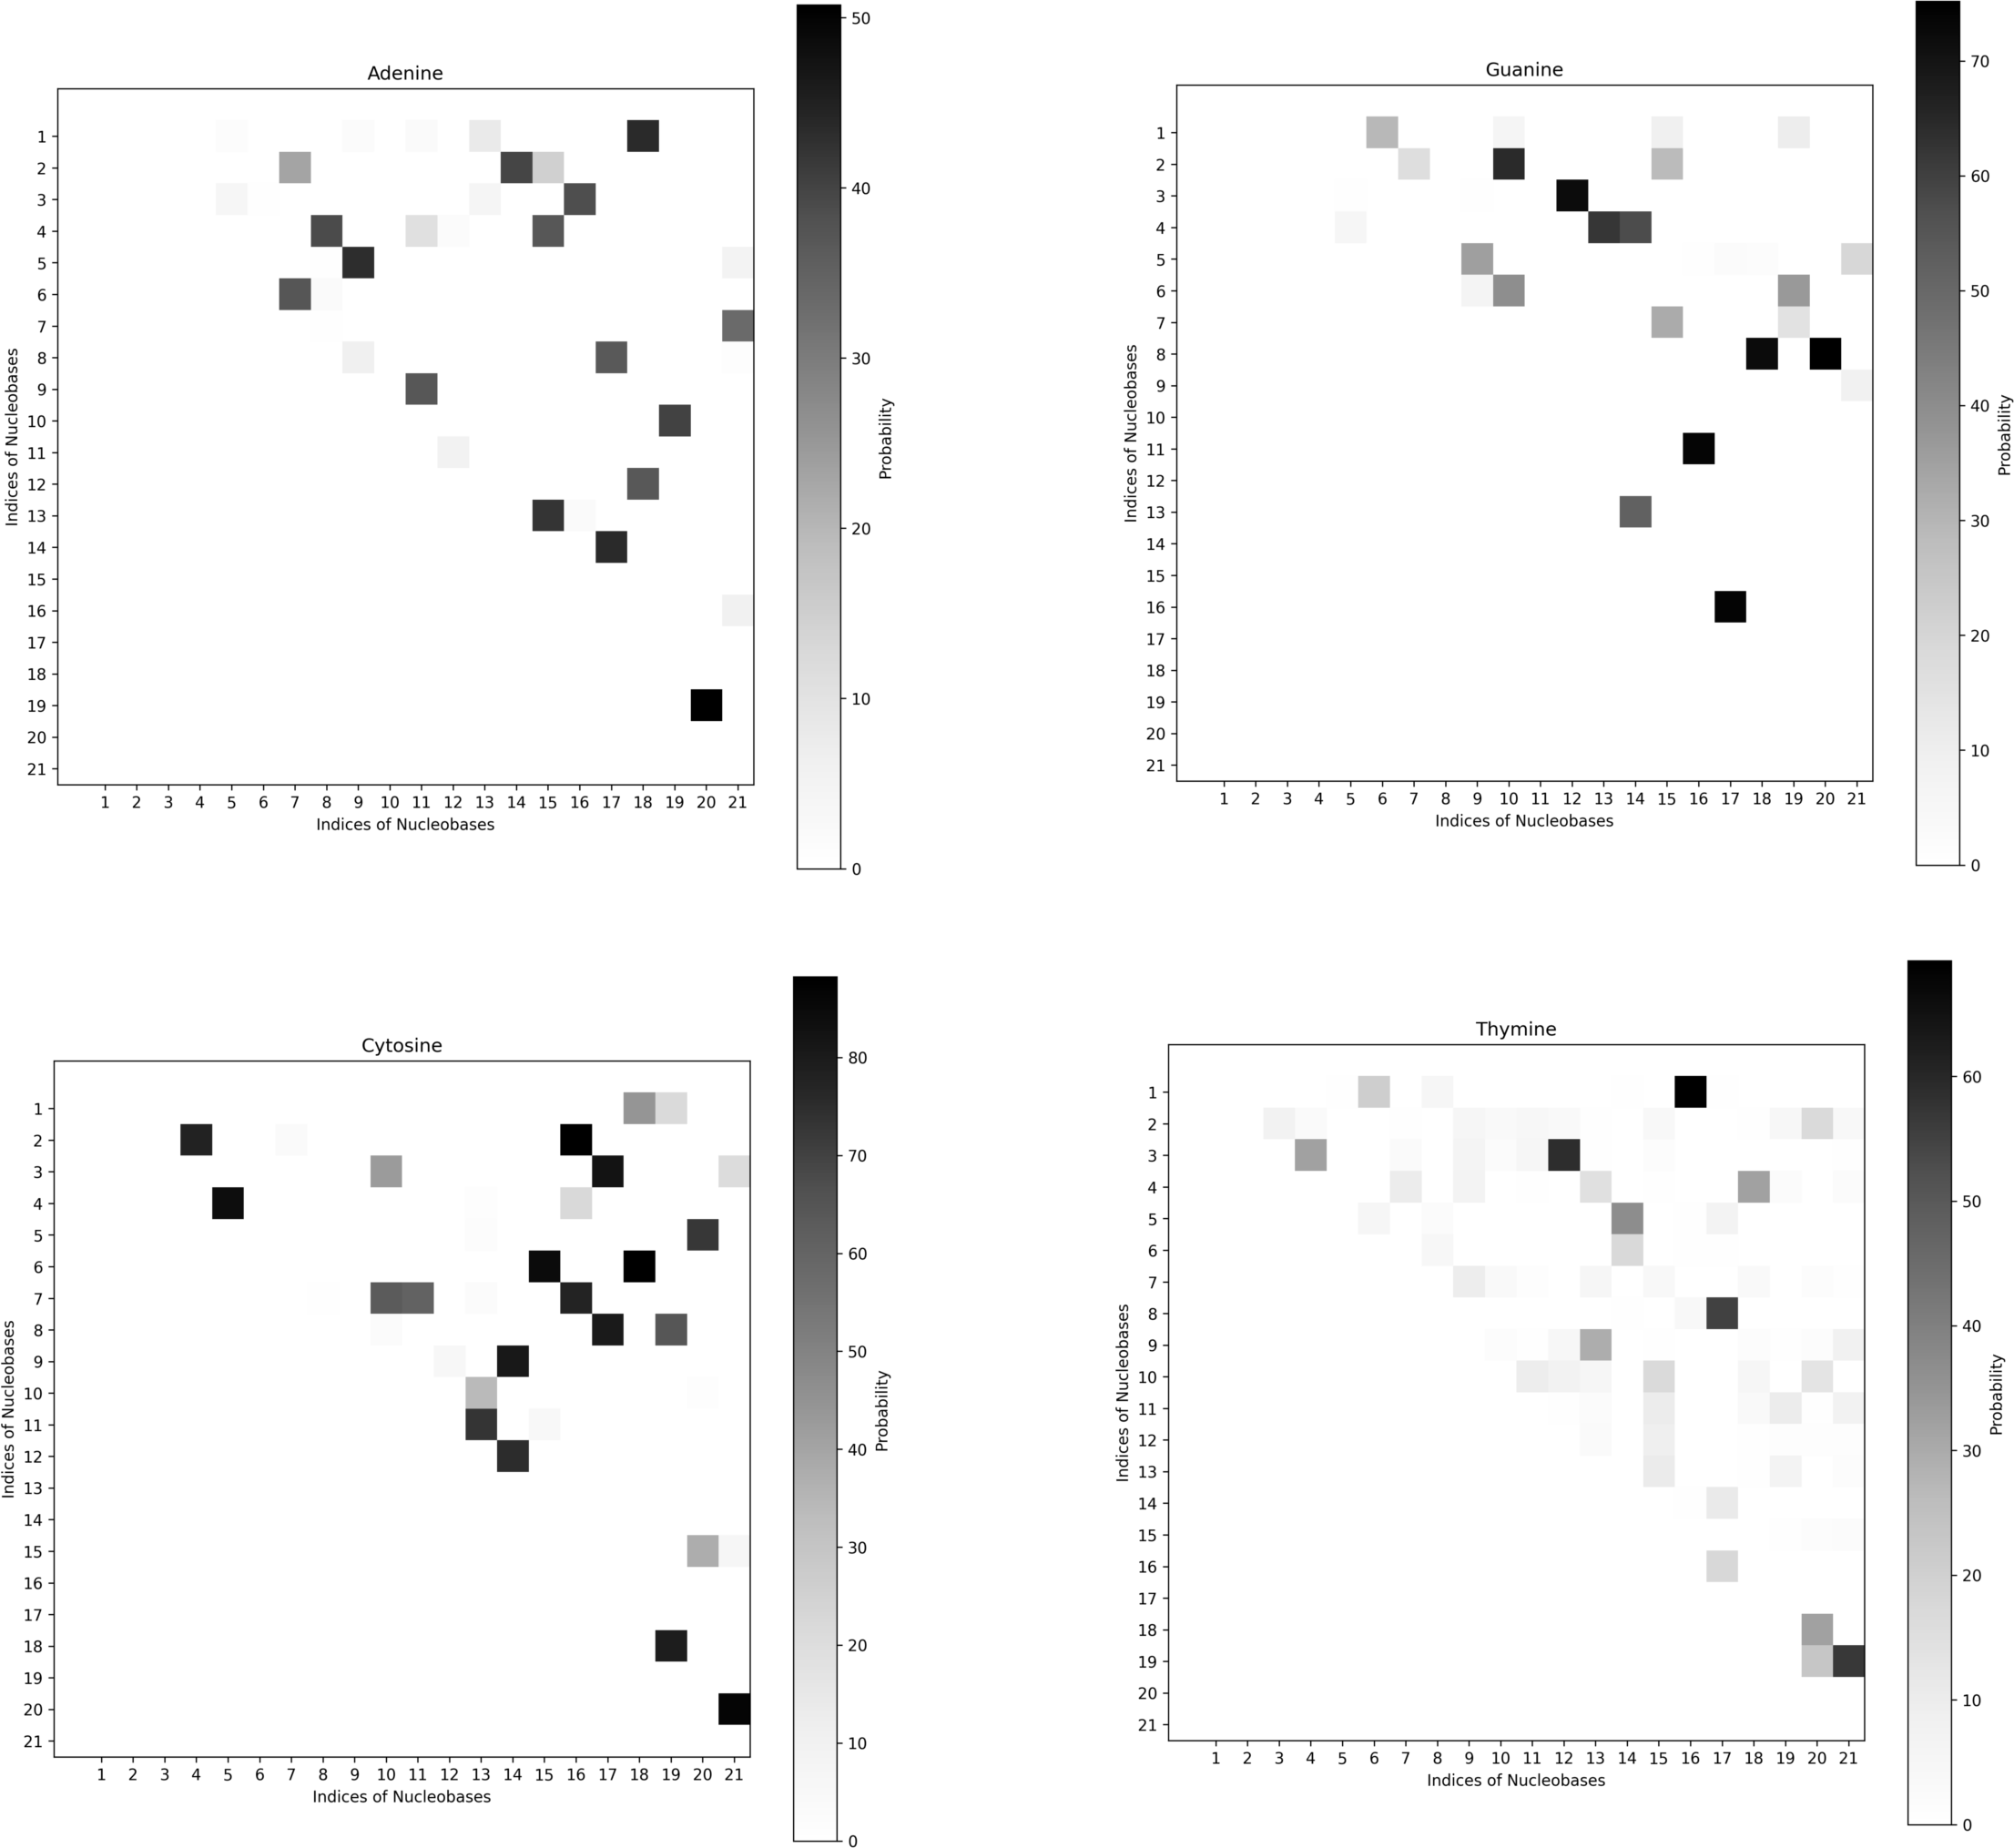
\includegraphics[width=\textwidth]{Appendix/Figures/A6_port.png}
    \caption[Heat-map plots depicting the probabilities of different hydrogen - bonded dimers within the simulation box for homogeneous nucleobase - graphene sheet Drude polarizable FF simulations]{Heat-map plots depicting the probabilities of different hydrogen - bonded dimers within the simulation box for homogeneous nucleobase - graphene sheet Drude polarizable FF simulations. Probabilities were calculated as number of occurances of each dimer in the simulation trajectory.}
\end{figure}

\begin{figure}
    \centering
    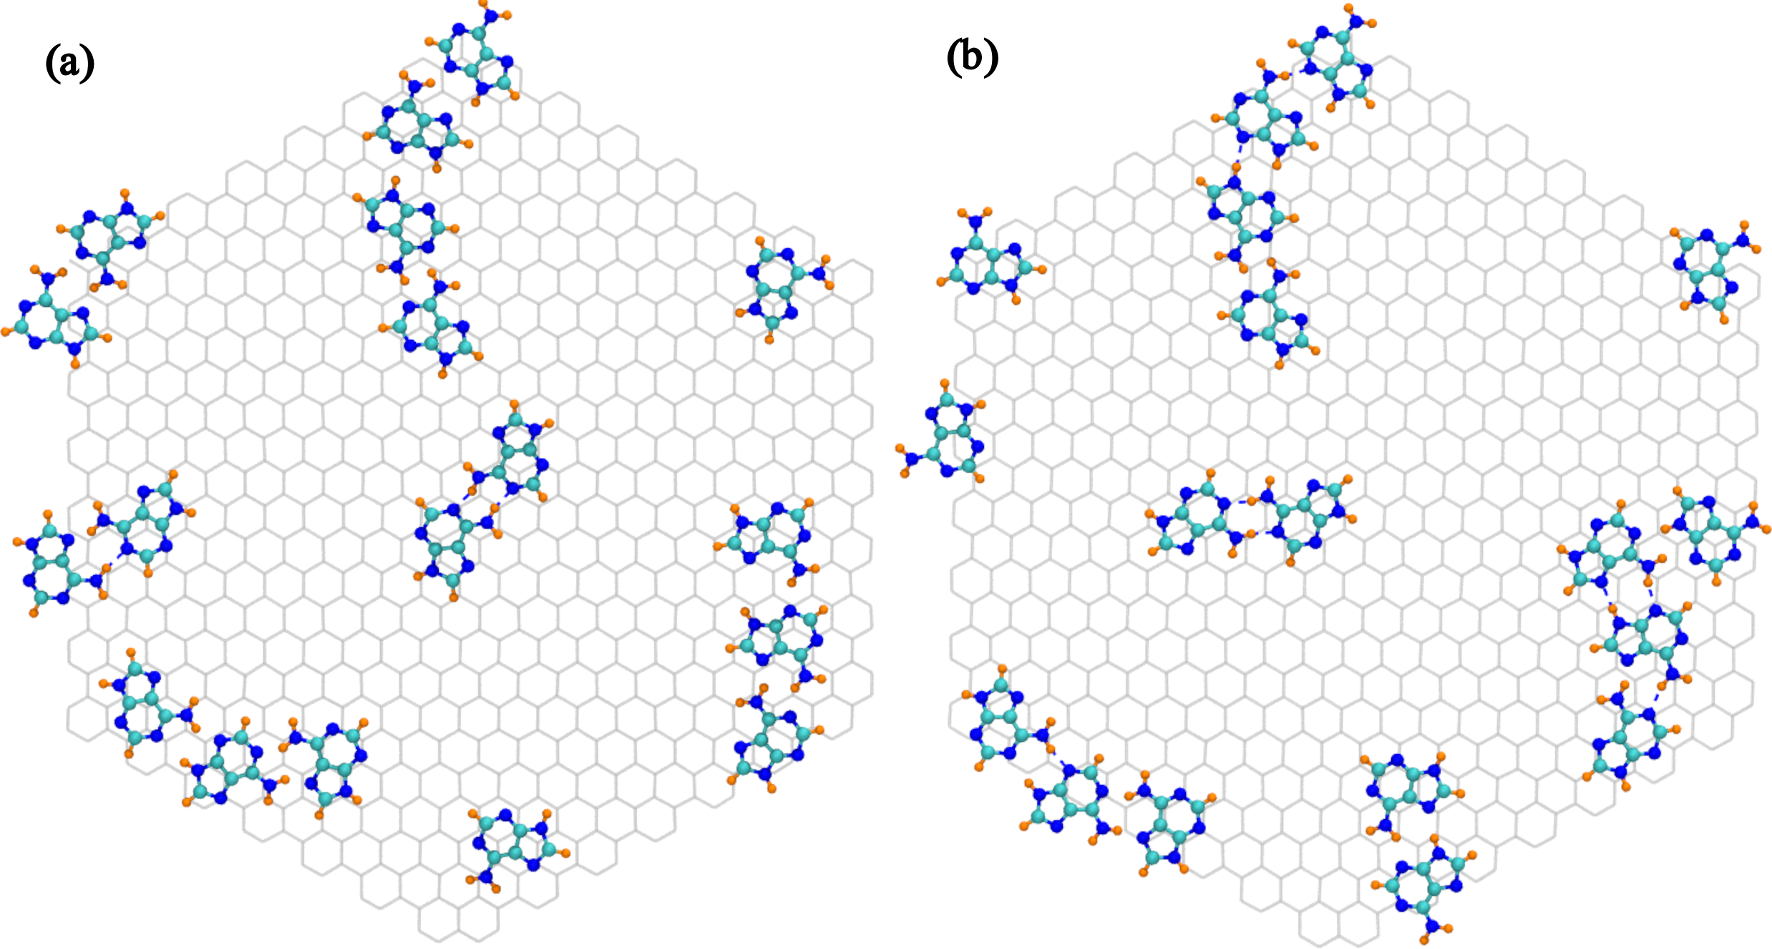
\includegraphics[width=\textwidth]{Appendix/Figures/A9_port.png}
    \caption[Representative image showing the self-organised higher-order structures formed by adenine on the graphene sheet]{Representative image showing the self-organised higher-order structures formed by adenine on the graphene sheet.}
\end{figure}

\begin{figure}
    \centering
    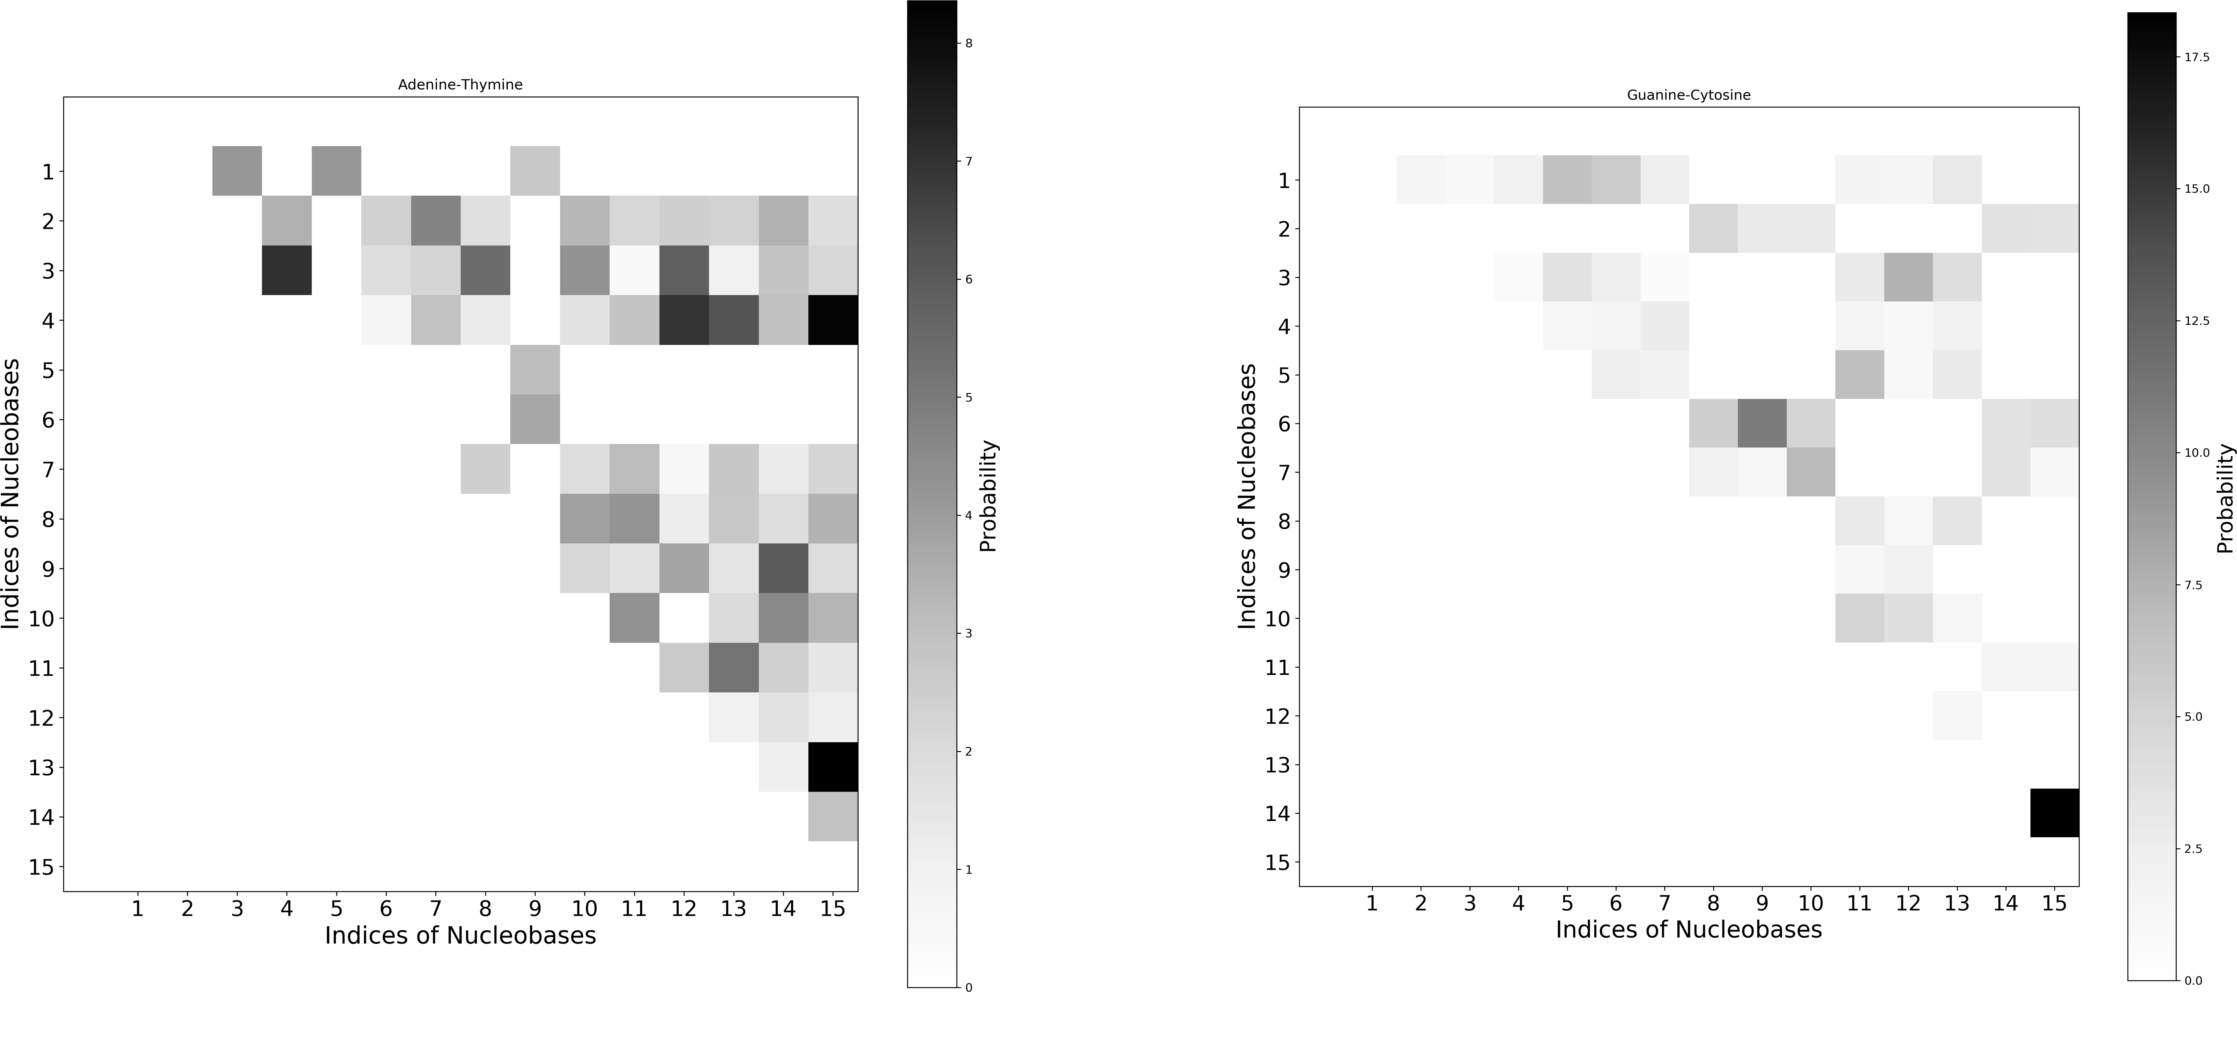
\includegraphics[width=\textwidth]{Appendix/Figures/A7_port.png}
    \caption[Heat-map plots depicting the probabilities of different hydrogen - bonded dimers within the simulation box for heterogeneous nucleobase - graphene sheet additive FF simulations]{Heat-map plots depicting the probabilities of different hydrogen - bonded dimers within the simulation box for heterogeneous nucleobase - graphene sheet additive FF simulations. Probabilities were calculated as number of occurances of each dimer in the simulation trajectory.}
\end{figure}

\begin{figure}
    \centering
    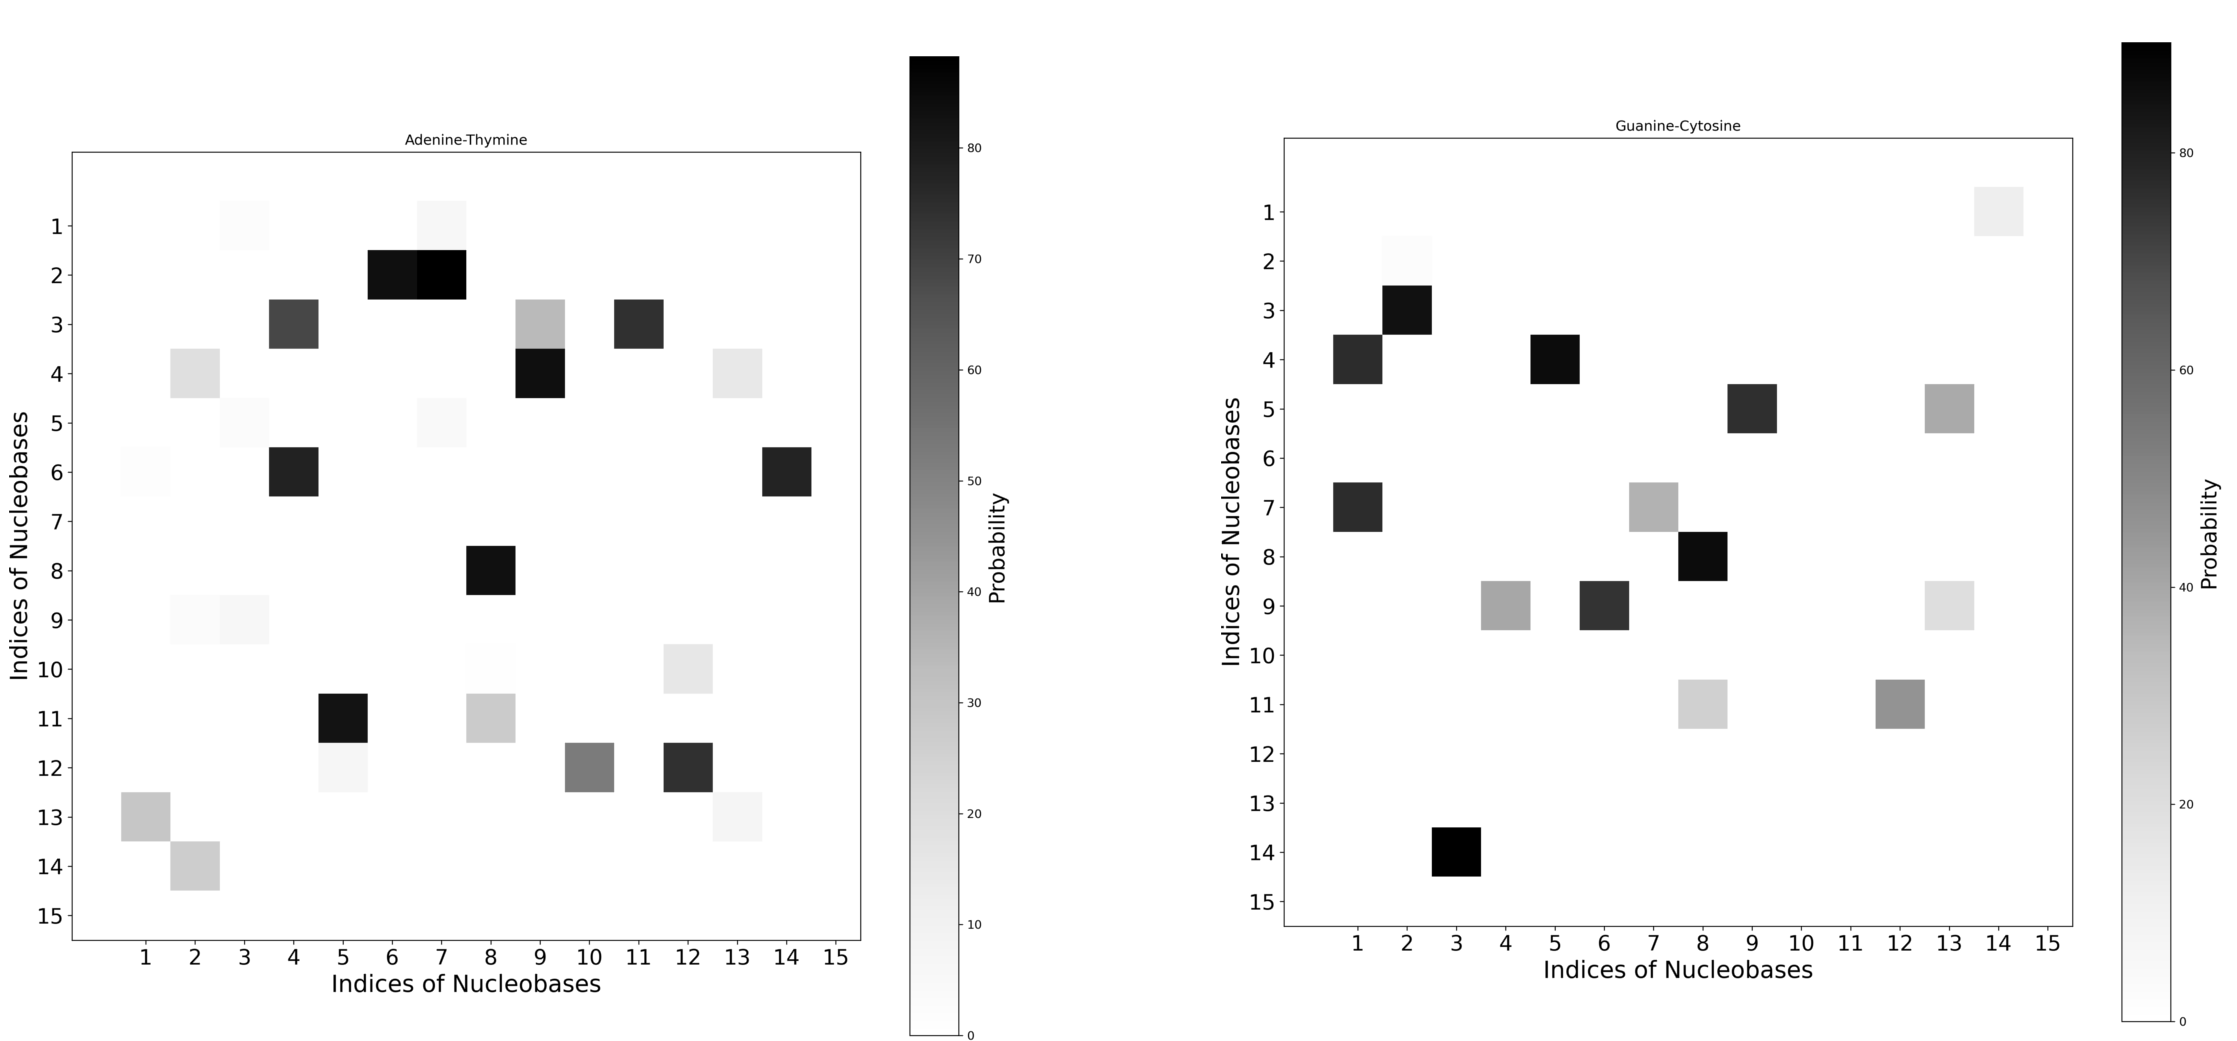
\includegraphics[width=\textwidth]{Appendix/Figures/A8_port.png}
    \caption[Heat-map plots depicting the probabilities of different hydrogen - bonded dimers within the simulation box for heterogeneous nucleobase - graphene sheet Drude polarizable FF simulations]{Heat-map plots depicting the probabilities of different hydrogen - bonded dimers within the simulation box for heterogeneous nucleobase - graphene sheet Drude polarizable FF simulations. Probabilities were calculated as number of occurances of each dimer in the simulation trajectory.}
\end{figure}